\section{ PlanesAndroid }

\subsection { Navigation }

The Android App is built around the so-called Drawer Navigation. This kind of navigation is based on a so-called Hamburger button which in case of the Planes App is displayed in the top left corner of the screen. Tapping on the button displays a list possible destinations in the application. These depend on whether the app is played in the Single Player or Multiplayer Mode. 

In the case of the Single Player App we have:
\begin{itemize}
\item Game
\item Videos
\item Settings
\item Info
\end{itemize}

For the Multiplayer App more screens are available:

\begin{itemize}
	\item Game
	\item Connect to Game
	\item Game Statistics
	\item Login
	\item Logout
	\item Register
	\item Delete User
	\item Videos
	\item Settings
	\item Info
\end{itemize}

When a screen is selected, a Fragment of the Fragment Class corresponding to the screen is loaded into the main layout of the application. 

\subsection { Android Concepts }

\subsubsection { Activity }

Activity is a central class in an Android app. In an activity the appearance of the app is defined through an XML layout. Also the behaviour of the app as response to variouse events in the app life cycle are defined in the activity.

For example the layout of the Planes Android app is as follows:

\begin{lstlisting}
<?xml version="1.0" encoding="utf-8"?>
	<androidx.drawerlayout.widget.DrawerLayout
	xmlns:android="http://schemas.android.com/apk/res/android"
	xmlns:app="http://schemas.android.com/apk/res-auto"
	android:id="@+id/drawer_layout"
	android:layout_width="match_parent"
	android:layout_height="match_parent"
	android:fitsSystemWindows="true">
		<RelativeLayout
		android:layout_width="match_parent"
		android:layout_height="match_parent">
			<androidx.appcompat.widget.LinearLayoutCompat
				android:id="@+id/coordinator_id"
				android:layout_width="match_parent"
				android:layout_height="match_parent"
				android:orientation="vertical"
				android:background="@drawable/background">
				<com.google.android.material.appbar.AppBarLayout
				android:layout_width="match_parent"
				android:layout_height="wrap_content"
				android:theme="@style/ThemeOverlay.AppCompat.Dark.ActionBar">
				<androidx.appcompat.widget.Toolbar
				android:id="@+id/toolbar"
				android:layout_width="match_parent"
				android:layout_height="?attr/actionBarSize"
				app:theme="@style/MyToolbarTheme"
				app:layout_scrollFlags="enterAlways|scroll" />
				</com.google.android.material.appbar.AppBarLayout>
				<androidx.appcompat.widget.LinearLayoutCompat
				android:id="@+id/main_content"
				android:layout_width="match_parent"
				android:layout_height="match_parent"
				app:layout_behavior="@string/appbar_scrolling_view_behavior"/>
			</androidx.appcompat.widget.LinearLayoutCompat>
			<ProgressBar
			android:id="@+id/ProgressBarBottom"
			android:layout_width="350dp"
			android:layout_centerInParent="true"
			android:layout_height="350dp"
			android:foregroundTint="?planesProgressBarColor"
			android:progressTint="?planesProgressBarColor"
			android:indeterminateTint="?planesProgressBarColor"
			android:visibility="invisible" />
			<TextView
			android:id="@+id/LoaderLabelBottom"
			android:layout_width="wrap_content"
			android:layout_height="wrap_content"
			android:layout_margin="10dip"
			android:layout_alignParentBottom="true"
			android:textSize="20sp"
			android:textStyle="bold"
			style="@style/CustomTextViewStyle"
			android:text="@string/loader_text"
			android:visibility="invisible"/>
		</RelativeLayout>
	<com.google.android.material.navigation.NavigationView
	android:id="@+id/nav_view"
	android:layout_width="wrap_content"
	android:layout_height="wrap_content"
	android:layout_gravity="left"
	android:background="@drawable/background"
	app:menu="@menu/main_menu"
	app:theme="@style/NavigationDrawerStyle"
	app:headerLayout="@layout/nav_header"
	/>
	</androidx.drawerlayout.widget.DrawerLayout>
\end{lstlisting}
 
This xml defines the layout as a special type of layout: DrawerLayout. This includes the NavigationView which is the part of the layout which appears when clicking on the Hamburger button and allows the navigation to the different screens of the app. The content of the main activity screen is contained inside a RelativeLayout. In this layout are included a general use Progress Bar which is normally disabled but appears when different network calls are being made. The RelativeLayout of the main screen contains the toolbar of the app and a placeholder for the different screens marked with the id main\_content.

\subsubsection { Life Cycle }

\tikzstyle{startstop} = [rectangle, rounded corners, minimum width=3cm, 
minimum height=1cm, text centered, draw=black, fill=red!30]
\tikzstyle{process} = [rectangle, minimum width=3cm, minimum height=1cm, text centered, draw=black, fill=orange!30]
\tikzstyle{comment} = [rectangle, minimum width=3cm, minimum height=1cm, text centered,
text width=4cm, draw=white, fill=white]
\tikzstyle{arrow} = [thick,->,>=stealth]

\begin{figure}
	\caption{Activity Life Cycle diagram as it is presented on the Android developer pages}
	\label{fig:activity_life_cycle}
	\centering
		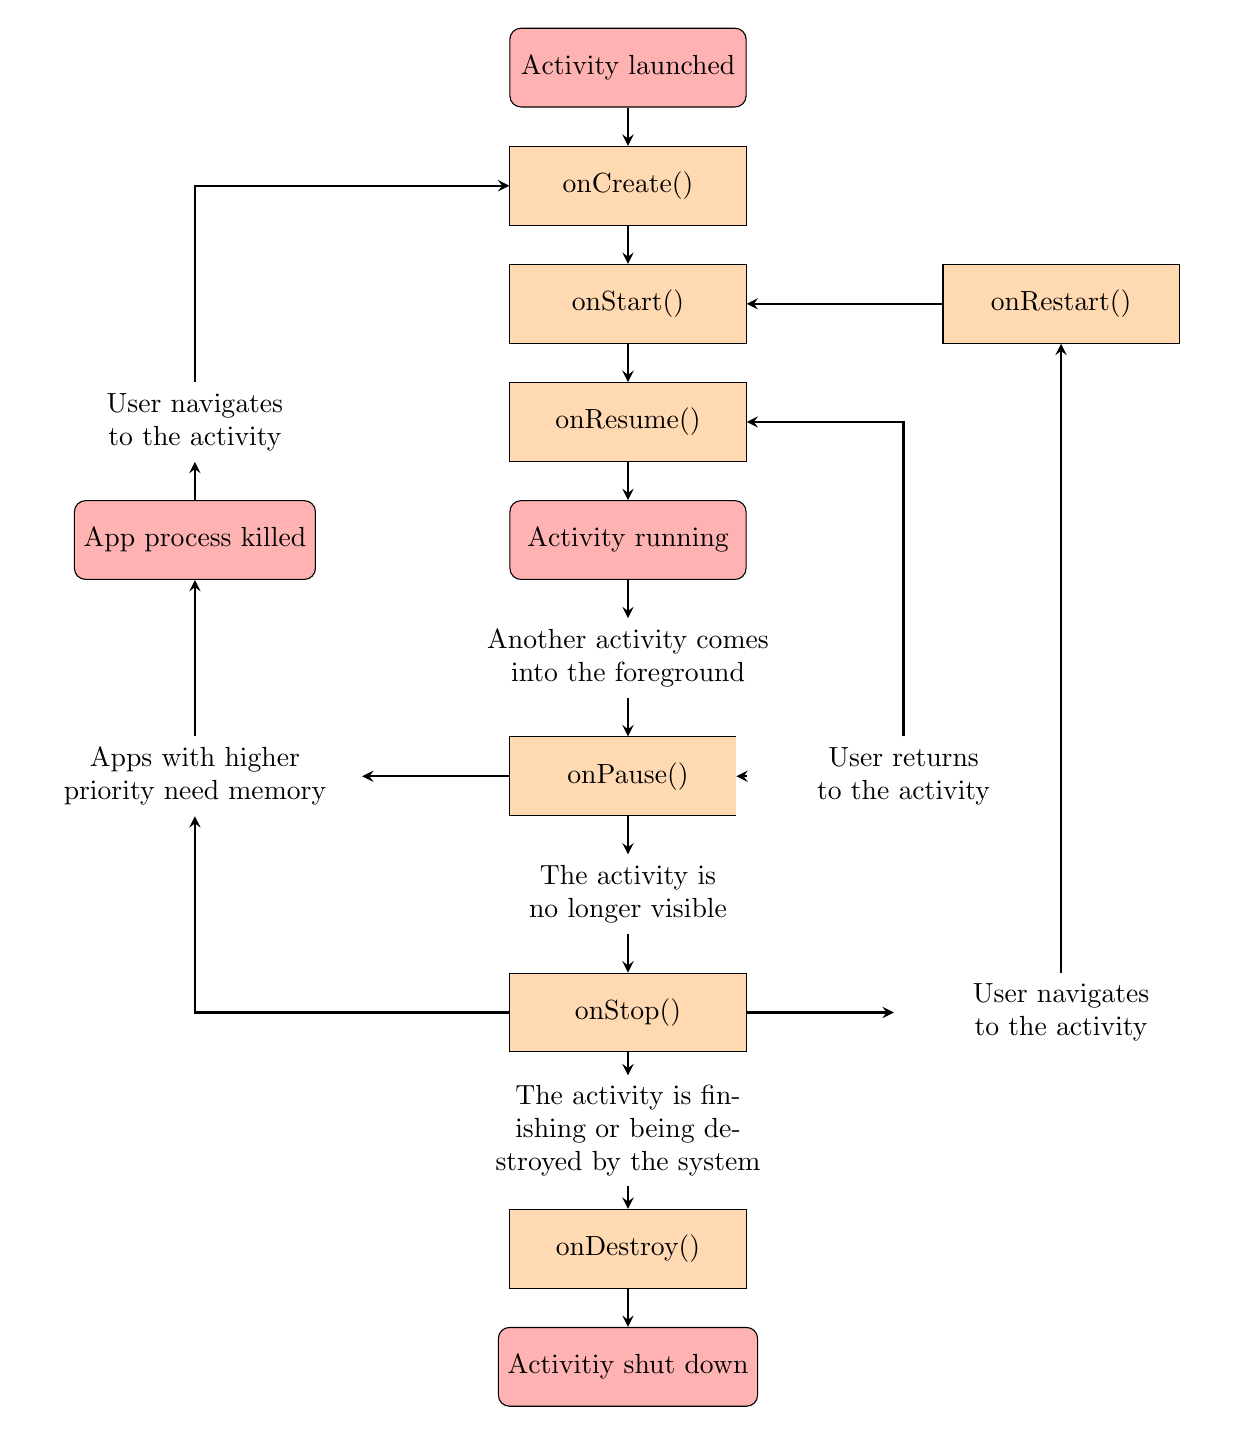
\begin{tikzpicture}[node distance=1.5cm]
			\node (start) [startstop] {Activity launched};
			\node (onCreate) [process, below of=start] {onCreate()};
			\node (onStart) [process, below of=onCreate] {onStart()};
			\node (onResume) [process, below of=onStart] {onResume()};
			\node (running) [startstop, below of=onResume] {Activity running};
			\node (commentOnPause) [comment, below of= running] {Another activity comes into the foreground};
			\node (onPause) [process, below of=commentOnPause] {onPause()};
			\node (commentOnStop) [comment, below of= onPause] {The activity is no longer visible};
			\node (onStop) [process, below of=commentOnStop] {onStop()};
			\node (commentOnDestroy) [comment, below of= onStop] {The activity is finishing or being destroyed by the system};
			\node (onDestroy) [process, below of=commentOnDestroy] {onDestroy()};
			\node (end) [startstop, below of=onDestroy] {Activitiy shut down};
			\node (onRestart) [process, right of=onStart, xshift=4cm] {onRestart()};
			\node (commentOnRestart) [comment, right of= onStop, xshift=4cm] {User navigates to the activity};
			\node (commentOnPauseRight) [comment, right of= onPause, xshift=2cm] {User returns to the activity};
			\node (commentOnPauseLeft) [comment, left of= onPause, xshift=-4cm] {Apps with higher priority need memory};
			\node (commentOnResumeLeft) [comment, left of= onResume, xshift=-4cm] {User navigates to the activity};
			\node (killed) [startstop, left of = running, xshift=-4cm] {App process killed};
			
			\draw [arrow] (start) -- (onCreate);
			\draw [arrow] (onCreate) -- (onStart);
			\draw [arrow] (onStart) -- (onResume);
			\draw [arrow] (onResume) -- (running);
			\draw [arrow] (running) -- (commentOnPause);
			\draw [arrow] (commentOnPause)  -- (onPause);
			\draw [arrow] (onPause) -- (commentOnStop);
			\draw [arrow] (commentOnStop) -- (onStop);
			\draw [arrow] (onStop) -- (commentOnDestroy);
			\draw [arrow] (commentOnDestroy) -- (onDestroy);
			\draw [arrow] (onDestroy) -- (end);
			\draw [arrow] (onRestart) -- (onStart);
			\draw [arrow] (onStop) -- (commentOnRestart);
			\draw [arrow] (commentOnRestart) -- (onRestart);
			\draw [arrow] (onPause) -- (commentOnPauseRight);
			\draw [arrow] (commentOnPauseRight) |- (onResume);
			\draw [arrow] (onPause) -> (commentOnPauseLeft);
			\draw [arrow] (onStop) -| (commentOnPauseLeft);
			\draw [arrow] (commentOnPauseLeft) -> (killed);
			\draw [arrow] (killed) -> (commentOnResumeLeft);
			\draw [arrow]  (commentOnResumeLeft) |- (onCreate);
			
		\end{tikzpicture}

\end{figure}

In figure \ref{fig:activity_life_cycle} one can see how various functions of the activity class are called depending in which state is the activity in following interaction with the user or with the Android operating system. The programmer has the possibilty to override these functions in order to customize the behaviour of the application.
\subsubsection { Fragment }